\section{Implementation, Integration \& Test Plan}
\subsection{Implementation Plan}

The system will be implemented using a thread strategy, which ensures that a core platform feature is fully functional before moving to the next one, delivering at each step of the implementation an intermediate product stakeholders can evaluate and validate. This strategy requires the identification of the system threads to be incrementally implemented and tested, based on the requirements outlined in the RASD.

\paragraph{T1: User Management} This thread allows users to create a new account via email and password, login to an existing one using their credentials, update their personal information, update their preferences, for instance sensor or GPS acquisition, and delete their account.

\paragraph{T2: Path Exploration} This thread allows the user to browse all the biking paths in a certain area, or only the ones connecting a departure and destination point, ranked by their status, and filtered based on their requirements, if any. The users can also visualize all the details regarding a given bike path, like obstacles along the way.

\paragraph{T3: Trip Management} This thread allows the user to visualize their global statistics, including total travelled distance, average speed and more, save bike paths as planned trips and visualize all their completed trips, with the relative statistics.

\paragraph{T4: Reporting} This thread allows the user to manage the lifecycle of manual and automatic reports obstacles. More specifically, allows the user to change the status of manual reports from \code{draft} to \code{published} and the status of automatic reports from \code{draft} to \code{validated} and then \code{published}.

\paragraph{T5: Alert Management} This thread allows the user to change their notification preferences and receive notifications about adverse weather or road conditions regarding their planned trips. 

\paragraph{T6: Integration Adapter} This thread has as its only objective to test the communication between the platform and the external map and weather services.

\paragraph{T7: Tracking Pipeline} This thread has as its only objective to test the interaction with the device of the user and the management of sensor and GPS data.

\subsection{Component Integration and Testing}

This testing plan follows an incremental strategy, where features are introduced and validated in stages. Each phase involves testing new components or extending the evaluation of previously integrated modules. We assume that the DBMS is fully functional at each step, so it's not depicted in this plan. Furthermore, external services are included in the diagram as we can test the communication between them and the adapters.

\begin{figure}[H]
    \centering
    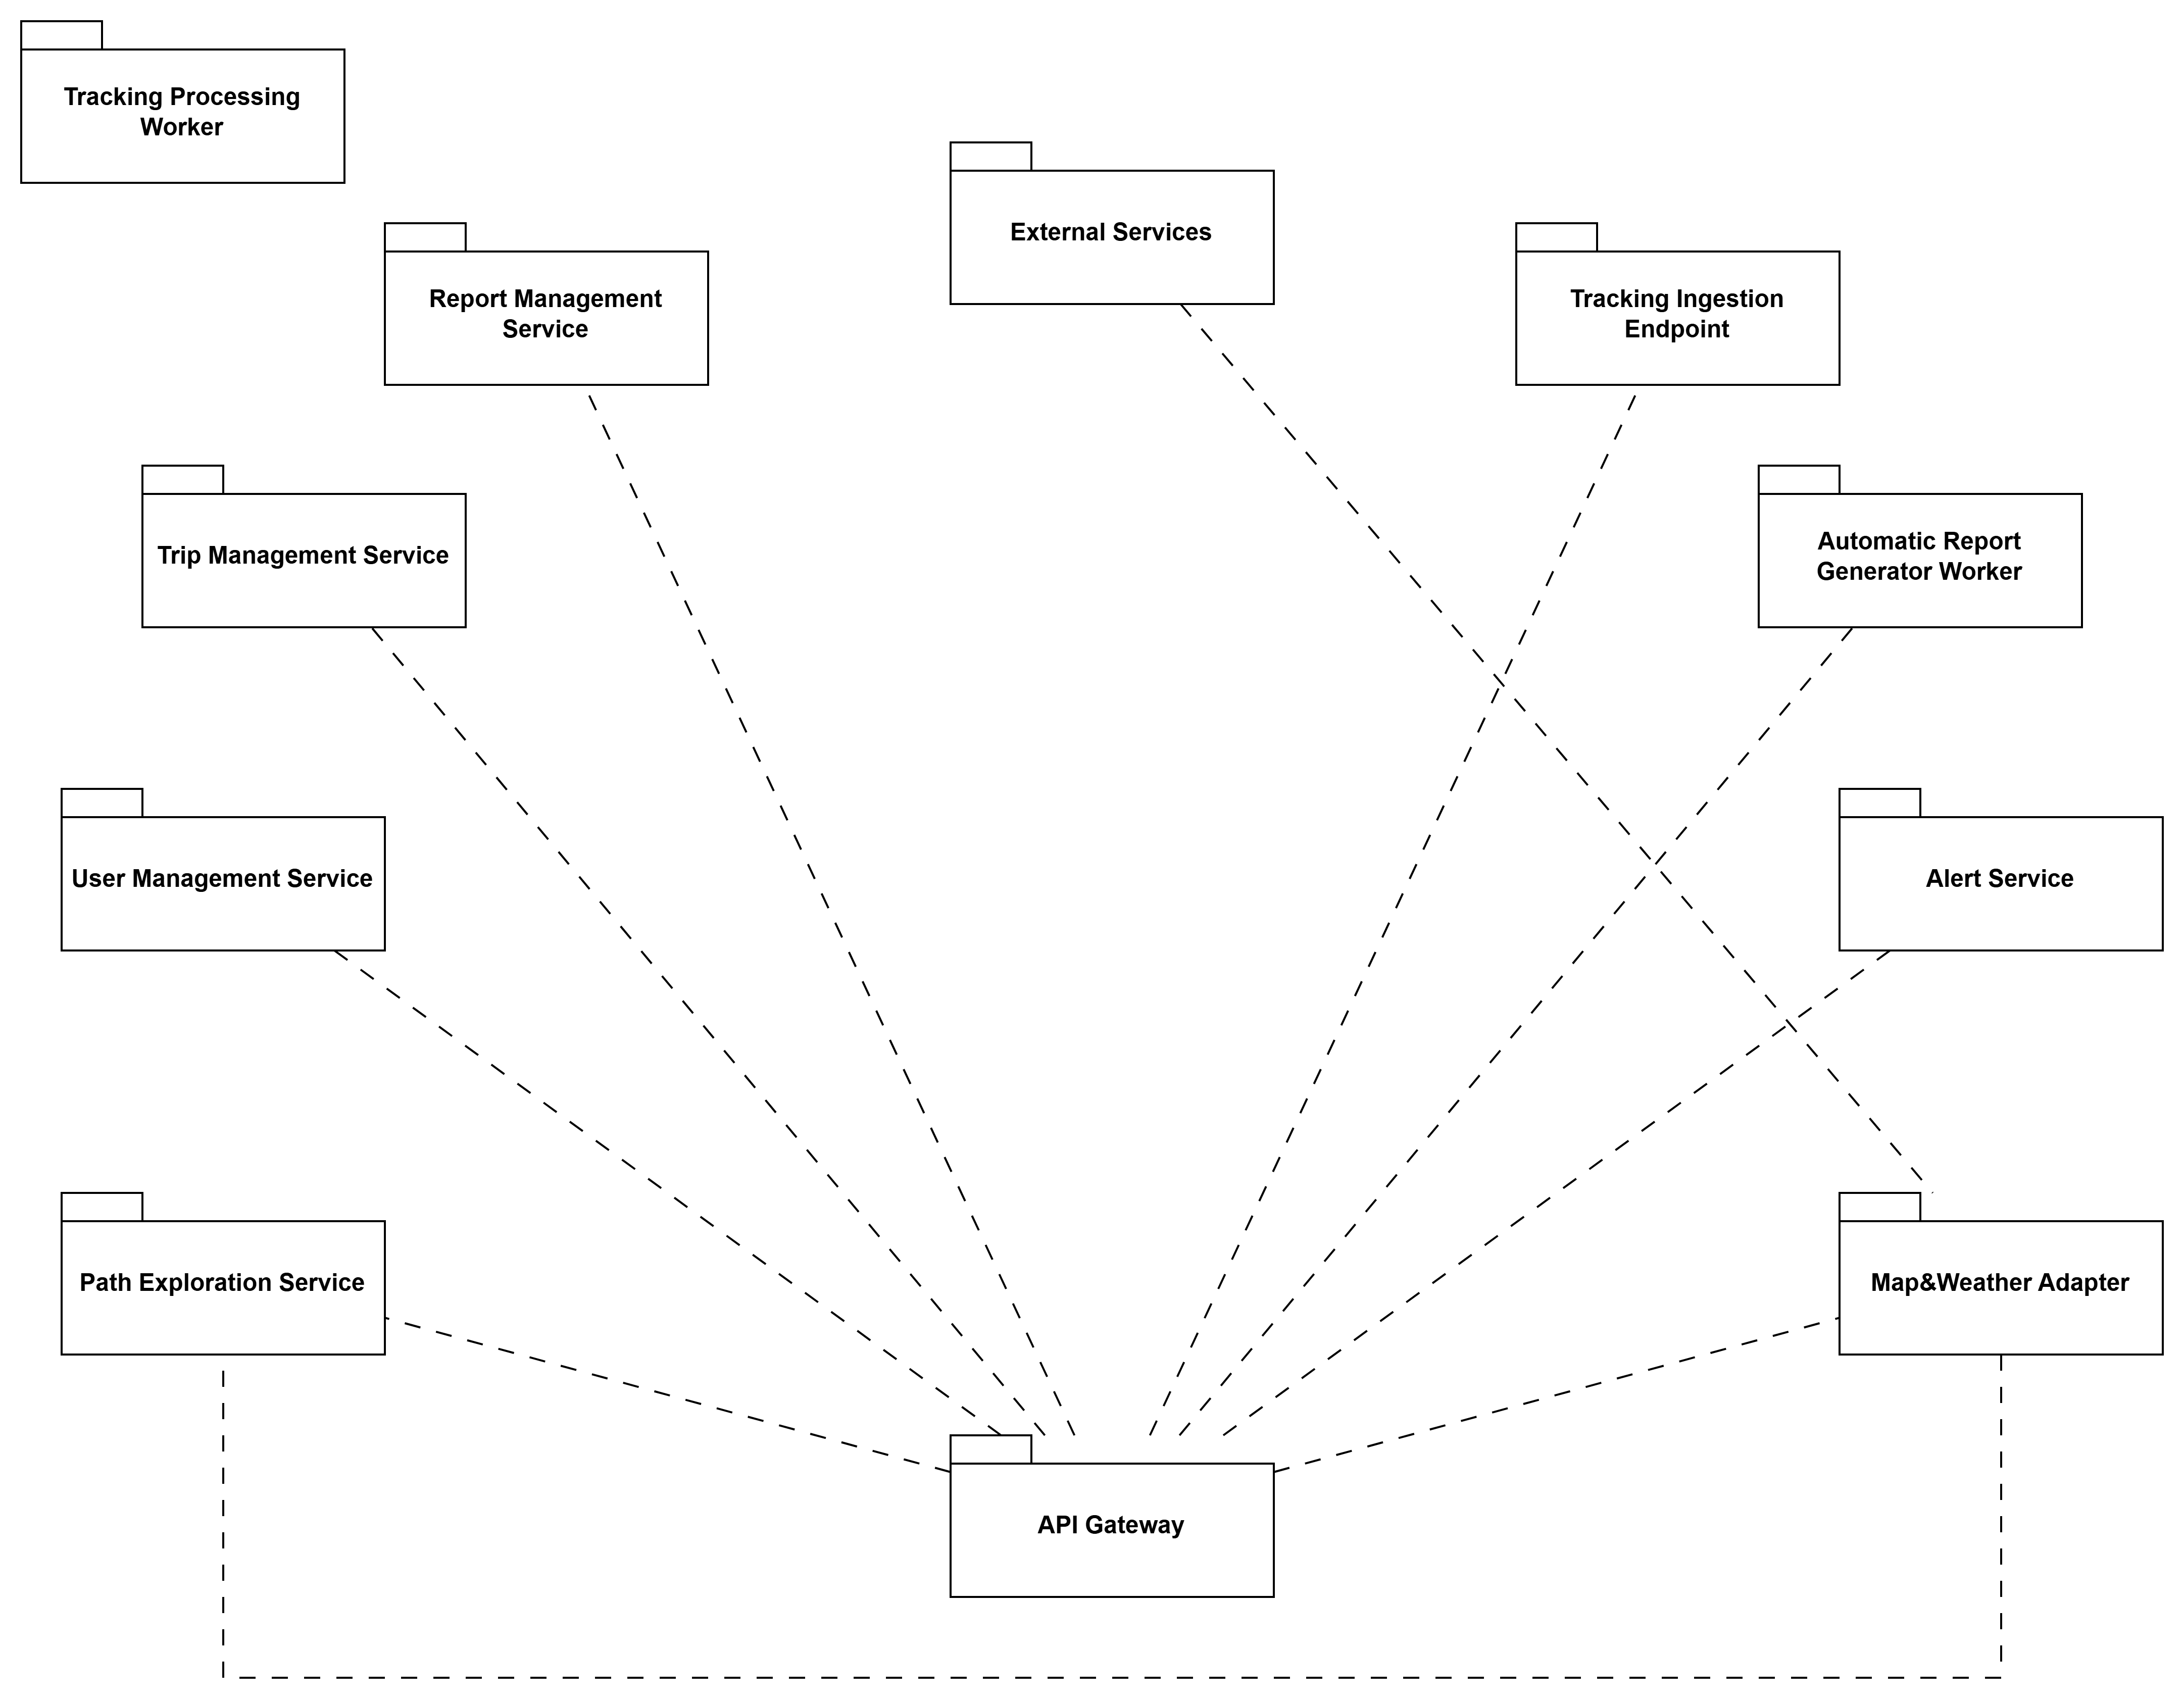
\includegraphics[width=0.9\linewidth]{DD//source//images//diagrams/test_plan_diagram.png}
    \caption{Test Plan Diagram.}
    \label{fig:test_plan_diagram}
\end{figure}

\paragraph{First Incremental Test}
This increment focuses on validating the core user onboarding functionalities, which are a prerequisite for accessing all other system features. The tested functionalities include user registration, authentication, profile data updates, and the management of consent and tracking preferences.
From an architectural perspective, this increment primarily involves: 
\begin{itemize}
    \item the client, which collects user input and initiates the interactions
    \item the API Gateway, which acts as the entry point and routes requests
    \item the User Management Component, which handles identity management, credential validation, profile persistence, and consent storage in compliance with GDPR requirements.
\end{itemize}

At the end of this increment, the system provides a fully functional and stable user management flow that can be used as a foundation for subsequent increments.

\paragraph{Second Incremental Test}
This increment validates the integration of external map services used to support path visualization within the system. The tested functionalities include the rendering of map views associated with bike paths and the correct handling of failure scenarios, such as timeouts or unavailability of the external map service, through fallback mechanisms.

The components involved in this increment are
\begin{itemize}
    \item the client, responsible for displaying the map to the user
    \item the API Gateway, which routes the requests
    \item the Path Exploration Service, which provides the path data to be visualized
    \item the Map \& Weather Integration component, which encapsulates communication with the external map service and enforces resilience policies.
\end{itemize}

This increment ensures that map-related features are robust and correctly isolated from external service failures before extending the system with additional context-aware functionalities.

\paragraph{Third Incremental Test}
This increment focuses on validating the core path exploration functionalities that do not depend on external services.

From an architectural standpoint, the client initiates the exploration requests, optionally involving the User Management Component when the user is authenticated, although these functionalities are also accessible to non-registered users. Requests are routed through the API Gateway to the Path Exploration Service, which retrieves and processes path data from the Persistence Store.

This increment ensures that the internal logic for path retrieval, filtering, and presentation is correct and stable before introducing contextual enrichments such as maps and weather information.

\paragraph{Fourth Incremental Test}
This increment validates the core functionalities related to trip management, focusing on trip planning and lifecycle handling. The tested features include the creation and storage of planned trips, the management of trip state transitions from planned to ongoing and completed, and the visualization of completed trips in the user’s trip history.

At the architectural level, the client allows the user to select a path and initiate trip-related actions, while the API Gateway routes the requests to the appropriate back-end services. The User Management Component ensures that only authenticated users can access these functionalities. The Path Exploration Service provides the selected path information required for planning, and the Trip Management Service manages trip persistence, state transitions, and history retrieval through interactions with the Persistence Store.

This increment establishes a stable foundation for advanced trip-related features, such as statistics computation, tracking, and reporting, which are introduced in subsequent increments.

\paragraph{Fifth Incremental Test}
This increment focuses on validating the functionalities related to trip statistics and trip history management. The tested features include the computation and visualization of performance statistics for completed trips, such as distance, duration, and average speed, as well as the soft deletion of trips from the user’s history.

The client enables the user to access statistics and request trip deletion, while the API Gateway routes these requests to the Trip Management Service. This service is responsible for computing statistics based on persisted trip data, enforcing consistency by excluding soft-deleted trips from aggregated views, and updating the Persistence Store accordingly.

By completing this increment, the system ensures that historical trip data is correctly managed and that performance analytics remain accurate and consistent.

\paragraph{Sixth Incremental Test}
This increment validates the tracking pipeline responsible for managing sensor and GPS data generated by the user’s device during a trip. The tested functionalities include the real-time ingestion of tracking data, its asynchronous processing, and the correct recording of trips based on the collected sensor information.

Architecturally, the User Device sends tracking data to the Tracking Ingestion Endpoint, which immediately publishes tracking events to the Event Bus without performing processing or persistence. The Tracking Processing Worker consumes these events, cleans and normalizes the data, and persists the processed tracking information in the Persistence Store. In parallel, the Trip Management Service updates the state of the trip (e.g., from ongoing to completed) based on tracking-related events and makes the recorded data available for subsequent statistics and reporting.

This increment ensures that continuous data streams are handled efficiently without impacting synchronous system operations, establishing the foundation for automatic reporting and alert evaluation.

\paragraph{Seventh Incremental Test}
This increment focuses on validating the reporting functionalities that allow the system to collect, manage, and publish information about bike paths. The tested features include the automatic generation of report drafts based on recorded tracking data, the validation of automatically generated reports by the user, the manual creation of reports, and the publication of validated reports.

From an architectural perspective, the Tracking Pipeline provides the processed tracking data required for automatic report generation. The Auto Report Generator Worker creates report drafts asynchronously, while the Reporting component manages the report lifecycle, including validation and publication. Once a report is published, the Path Exploration Service is updated with the new path-related information (e.g., obstacles or hazards), ensuring that the inventory reflects the most recent and reliable data.

This increment ensures that reporting workflows are correctly integrated with both tracking and path exploration, enabling accurate enrichment of path information and supporting subsequent alert evaluation.

\paragraph{Eighth Incremental Test}
This increment validates the alert management functionalities related to obstacle detection and contextual risk evaluation. The tested features include the evaluation of newly published reports, the assessment of weather conditions impacting planned trips, and the delivery of alert notifications to affected users.

At the architectural level, the Reporting component publishes events when new reports are validated and published. These events, together with contextual updates such as weather information, are consumed by the Alert Evaluation Worker, which evaluates severity thresholds and determines whether planned trips are impacted. The Trip Management Service provides information about users’ planned trips and their associated paths, allowing alerts to be targeted only to relevant users. When critical conditions are detected, the alert management logic triggers notifications in an event-driven manner, without relying on continuous polling.

This increment ensures that alert evaluation and notification mechanisms are reactive, decoupled, and correctly integrated with reporting and trip management, completing the system’s support for safety-critical user notifications.

\subsection{System Testing}
The following validation and verification procedures are executed after all platform functionalities are verified:
\begin{itemize}
    \item Functional Testing: validates the system against the Requirement Analysis and Specification Document to ensure all business threads operate as intended.
    \item Performance Testing: evaluates non-functional requirements to identify implementation inefficiencies that could hinder system speed or stability.
    \item Usability Testing: focuses on accessibility and user interaction, ensuring the BBP platform remains intuitive and user-friendly for its broad audience.
    \item Load Testing: simulates expected traffic volumes to verify that the system maintains efficiency and stability under concurrent user activity.
    \item Stress Testing: pushes the system beyond its normal operational limits to identify breaking points and evaluate how it recovers from extreme conditions.
\end{itemize}